\documentclass[a4paper,11pt,exos]{nsi} % COMPILE WITH DRAFT
\usepackage{pifont}
\pagestyle{empty}

\begin{document}
\classe{\premiere spé}
\titre{Corrigé - Inéquations(2)}
\maketitle


Résoudre dans $\R$ les inéquations suivantes :
\begin{multicols}{2}
    \begin{enumerate}[itemsep=1em]
        \item $-5x^2+10x-6> 0$
	    \item $-2x^2+12x-10>0$
	    \item $-x^2-x+2< 0$
	    \item $-x^2-4x-9\leqslant 0$
	    \item $4x^2+8x-12>0$
	    \item $-x^2+2x+3\geqslant 0$
    \end{enumerate}
\end{multicols}

\begin{enumerate}[itemsep=1em]
    \item Soit $P$ le polynôme défini pour tout $x$ de $\mathbb R$ par $P(x)=-5x^2+10x-6$.\\On cherche à résoudre $P(x)> 0$.\\Pour cela, on cherche ses racines éventuelles.\\$\Delta = 10^2-4\times(-5)\times(-6)=-20$\\$\Delta<0$ donc le polynôme $P$ n'admet pas de racine.\\ Il est toujours du signe de $a=-5<0$, donc $P(x)<0$ pour tout $x$ de $\mathbb{R}$.\\ On en déduit $S=\emptyset$.
    
    \item Soit $P$ le polynôme défini pour tout $x$ de $\mathbb R$ par $P(x)=-2x^2+12x-10$.\\On cherche à résoudre $P(x)>0$.\\Pour cela, on cherche ses racines éventuelles.\\$\Delta = 12^2-4\times(-2)\times(-10)=64$\\$\Delta>0$ donc le polynôme admet deux racines : $x_1 = \dfrac{-b-\sqrt{\Delta}}{2a}$ et $x_2 = \dfrac{-b+\sqrt{\Delta}}{2a}$.\\$x_1 =\dfrac{-12-\sqrt{64}}{-4}=1$\\$x_2 =\dfrac{-12+\sqrt{64}}{-4}=5$\\On sait qu'un polynôme du second degré est du signe de $a$ à l'extérieur de ses racines.\\Comme $a=-2<0$\\on en déduit le signe du polynôme dans un tableau de signes :\\
    \begin{tikzpicture}[baseline, scale=0.5]
        \tkzTabInit[lgt=8,deltacl=0.8,espcl=5]{ $x$ / 2, $-2x^2+12x-10$ / 2}{ $-\infty$, 1, 5, $+\infty$}
        \tkzTabLine{  , -, z, +, z, -}
        \end{tikzpicture}
    \\[.5em] 
    Finalement $S=]1;5[$.
    
    \item Soit $P$ le polynôme défini pour tout $x$ de $\mathbb R$ par $P(x)=-x^2-x+2$.\\On cherche à résoudre $P(x)< 0$.\\Pour cela, on cherche ses racines éventuelles.\\$\Delta = (-1)^2-4\times(-1)\times2=9$\\$\Delta>0$ donc le polynôme admet deux racines : $x_1 = \dfrac{-b-\sqrt{\Delta}}{2a}$ et $x_2 = \dfrac{-b+\sqrt{\Delta}}{2a}$.\\$x_1 =\dfrac{1-\sqrt{9}}{-2}=-2$\\$x_2 =\dfrac{1+\sqrt{9}}{-2}=1$\\On sait qu'un polynôme du second degré est du signe de $a$ à l'extérieur de ses racines.\\Comme $a=-1<0 :$\\On peut résumer le signe du polynôme dans un tableau de signes :\\
    \begin{tikzpicture}[baseline, scale=0.5]
        \tkzTabInit[lgt=8,deltacl=0.8,espcl=5]{ $x$ / 2, $-x^2-x+2$ / 2}{ $-\infty$, -2, 1, $+\infty$}
        \tkzTabLine{  , -, z, +, z, -}
        \end{tikzpicture}
    \\[.5em]
    Finalement $S=]-\infty;-2[\cup]1;+\infty[$.
    
    \item Soit $P$ le polynôme défini pour tout $x$ de $\mathbb R$ par $P(x)=-x^2-4x-9$.\\On cherche à résoudre $P(x)\leqslant 0$.\\Pour cela, on cherche ses racines éventuelles.\\$\Delta = (-4)^2-4\times(-1)\times(-9)=-20$\\$\Delta<0$ donc le polynôme $P$ n'admet pas de racine.\\ Il est toujours du signe de $a=-1<0$, donc $P(x)<0$ pour tout $x$ de $\mathbb{R}$.\\ On en déduit $S=\mathbb{R}$.
    
    \item Soit $P$ le polynôme défini pour tout $x$ de $\mathbb R$ par $P(x)=4x^2+8x-12$.\\On cherche à résoudre $P(x)>0$.\\Pour cela, on cherche ses racines éventuelles.\\$\Delta = 8^2-4\times4\times(-12)=256$\\$\Delta>0$ donc le polynôme admet deux racines : $x_1 = \dfrac{-b-\sqrt{\Delta}}{2a}$ et $x_2 = \dfrac{-b+\sqrt{\Delta}}{2a}$.\\$x_1 =\dfrac{-8-\sqrt{256}}{8}=-3$\\$x_2 =\dfrac{-8+\sqrt{256}}{8}=1$\\On sait qu'un polynôme du second degré est du signe de $a$ à l'extérieur de ses racines.\\Comme $a=4>0$\\on en déduit le signe du polynôme dans un tableau de signes :\\
    \begin{tikzpicture}[baseline, scale=0.5]
        \tkzTabInit[lgt=8,deltacl=0.8,espcl=5]{ $x$ / 2, $4x^2+8x-12$ / 2}{ $-\infty$, -3, 1, $+\infty$}
        \tkzTabLine{  , +, z, -, z, +}
        \end{tikzpicture}
    \\[.5em]
    Finalement $S=]-\infty;-3[\cup]1;+\infty[$.
    
    \item Soit $P$ le polynôme défini pour tout $x$ de $\mathbb R$ par $P(x)=-x^2+2x+3$.\\On cherche à résoudre $P(x)\geq 0$.\\Pour cela, on cherche ses racines éventuelles.\\$\Delta = 2^2-4\times(-1)\times3=16$\\$\Delta>0$ donc  le polynôme admet deux racines : $x_1 = \dfrac{-b-\sqrt{\Delta}}{2a}$ et $x_2 = \dfrac{-b+\sqrt{\Delta}}{2a}$.\\$x_1 =\dfrac{-2-\sqrt{16}}{-2}=-1$\\$x_2 =\dfrac{-2+\sqrt{16}}{-2}=3$\\On sait qu'un polynôme du second degré est du signe de $a$ à l'extérieur de ses racines.\\Comme $a=-1<0$, \\on peut résumer le signe du polynôme dans un tableau de signes :\\
    \begin{tikzpicture}[baseline, scale=0.5]
        \tkzTabInit[lgt=8,deltacl=0.8,espcl=5]{ $x$ / 2, $-x^2+2x+3$ / 2}{ $-\infty$, -1, 3, $+\infty$}
        \tkzTabLine{  , -, z, +, z, -}
        \end{tikzpicture}
    \\[.5em]
    Finalement $S=[-1;3]$.
    \end{enumerate}

\end{document}